\documentclass{beamer}
% Set the fonts of the document
\usepackage{inconsolata} % Monospace font
\usepackage{helvet} % Sans-serif font
\usepackage[
    libertine, % do not override the sans-serif-font
    tt = false % do not override the monospace font
]{libertine} % Main font (serif)

\usepackage[
    top = 3cm,
    bottom = 3cm,
    left = 2.5cm,
    right = 2.5cm
]{geometry}

\usepackage[english]{babel}
\usepackage{xspace}
\usepackage{booktabs}
\usepackage{enumitem}
\usepackage[xcolor]{mdframed}
\usepackage{amsmath}
\usepackage{amssymb}
\usepackage{amsthm}
\usepackage{mathrsfs}
\usepackage{stmaryrd}
\usepackage{float}
\usepackage{listings}
\usepackage{parskip}
\usepackage[
    labelfont = {small, bf},
    textfont = {small}
]{caption}
\usepackage{subcaption}
\usepackage{circledsteps}
\usepackage{hyperref}

% ====================================================================

\newcommand{\eg}{e.g.,\xspace}
\newcommand{\ie}{i.e.\xspace}
\newcommand{\etal}{\textit{et~al.}\xspace}

\newcommand{\todo}[1]{{\centering\textbf{\textcolor{red}{[TODO : #1]}}\xspace}}

\newcommand{\vsc}{Visual Studio Code\xspace}

\DeclareRobustCommand{\iLaTeX}{\mbox{{{\itshape i}-\hspace{-0.25mm}}\LaTeX{}}}

% Document title
\newcommand{\makedoctitle}[1]{%
\begin{center}
    \color{black!75}
    {\Large{Longitudinal study of \iLaTeX}} \\
    \noindent\rule{12cm}{0.4pt} \\[1.5em]
    \color{black}
    {\Huge{#1}} \\[0.5em]
    % \noindent\rule{16cm}{0.4pt}
\end{center}
}

% Custom framed environments
\newmdenv[
    linecolor = red!50!black,
    backgroundcolor = red!2,
    skipabove = 1em,
    skipbelow = 1em,
    innertopmargin = 1em,
    innerbottommargin = 1em,
    frametitle = {Warning},
    frametitlebackgroundcolor = red!5,
    % startinnercode = \centering\bgroup,
    % endinnercode = \egroup
    nobreak = true
]{warning}

\newmdenv[
    linecolor = blue!50!black,
    backgroundcolor = blue!2,
    skipabove = 1em,
    skipbelow = 1em,
    innertopmargin = 1em,
    innerbottommargin = 1em,
    frametitle = {Good to know},
    frametitlebackgroundcolor = blue!5,
    % startinnercode = \centering\bgroup,
    % endinnercode = \egroup
    nobreak = true
]{info}

\newmdenv[
    linecolor = green!50!black,
    backgroundcolor = green!2,
    skipabove = 1em,
    skipbelow = 1em,
    innertopmargin = 1em,
    innerbottommargin = 1em,
    frametitle = {Example},
    frametitlebackgroundcolor = green!5,
    % startinnercode = \centering\bgroup,
    % endinnercode = \egroup,
    % nobreak = true
]{example}

% Style of code blocks
\lstdefinestyle{custom-latex}{
    language={[LaTeX]TeX},
    backgroundcolor=\color{white},
    commentstyle=\color{black!50},
    keywordstyle=\color{green!50!black},
    numberstyle=\tiny\color{red!50!black},
    stringstyle=\color{blue!50!black},
    basicstyle=\ttfamily\small,
    breakatwhitespace=false,         
    breaklines=true,
    keepspaces=true,
    numbers=none,
    tabsize=4,
    aboveskip={1em},
    belowskip={0.7em}
}

\lstdefinestyle{custom-latex-example}{
    language={[LaTeX]TeX},
    commentstyle=\color{black!50},
    keywordstyle=\color{green!50!black},
    numberstyle=\tiny\color{red!50!black},
    stringstyle=\color{blue!50!black},
    basicstyle=\ttfamily\footnotesize,
    breakatwhitespace=false,         
    breaklines=true,
    keepspaces=true,
    numbers=none,
    tabsize=4,
    aboveskip={1em},
    belowskip={-1ex}
}

% Description of a command/environment (for the cheat sheet)
\newcommand{\commanddesc}[1]{{\color{black!80}{#1}}}


% Command to produce a circled number to reference a step represented in a figure
\definecolor{FigStepColor}{HTML}{BC43F0}

\DeclareRobustCommand{\figstep}[1]{%
    \Circled[%
        inner color=white,%
        outer color=white,%
        fill color=FigStepColor%
    ]{\sffamily\textbf{#1}}%
}

\title{Presentation about Covid-19}
\subtitle{\iLaTeX{} evaluation}
\date{}

\begin{document}

\maketitle


%%%%%%%%%%%%%%%%%%%%%%%%%%%%%%%% START EDITING HERE

\begin{frame}{Title of frame 1}
  \centering
  \iincludegraphics[width=264px, height=172px, clip, trim=0px 0px 0px 30px]{img/matplotlib-graph.png}
\end{frame}



\begin{frame}{Title of frame 2}
    \centering
	\begin{itabular}{lc}
		\hline
		Designs& ArIc(in \%)\\ 
		\hline
		$A_1,\delta_{2}$&$41.44$\\
		$A_2,A_3,\delta_{3},\delta_{4}$&$1.57$\\
		$A_4$&$0.19$\\
		$\delta_1$&$45.45$\\
		$\delta_{5c}$&$2.28$\\
		$\delta_{10a}$&$3.31$\\
		$\delta_{10b},\delta_{15a},\delta_{15b}$&$3.94$\\
		$\delta_{10c}$&$2.38$\\
		$\delta_{15c}$&$1.04$\\
		$\delta_{5a},\delta_{5b}$&$3.00$\\
		xxx & yyy \\
		\hline
	\end{itabular}
\end{frame}



\begin{frame}{Title of frame 3}
    \small
    \begin{gridlayout}{\textwidth}{0.67\textwidth}
      \begin{row}{0.627}
        \begin{cell}{0.446}
          The size of a frame is actually the “paper size” of abeamerpresentation, and it is variable. By default, itamounts to 128 mm by 96 mm. The aspect ratio of this size is 4:3, which is exactly what most beamers offerthese days. It is the job of the presentation program (likeacroread,xpdf,okularorevince) to display theslides at full screen size.
        \end{cell}
        \begin{cell}{0.077}
          ~
        \end{cell}
        \begin{cell}{0.475}
          The size of a frame is actually the “paper size” of abeamerpresentation, and it is variable. By default, itamounts to 128 mm by 96 mm. The aspect ratio of this size is 4:3, which is exactly what most beamers offerthese days. It is the job of the presentation program (likeacroread,xpdf,okularorevince) to display theslides at full screen size.
        \end{cell}
      \end{row}
      \begin{row}{0.373}
        \begin{cell}{0.445}
          \centering
          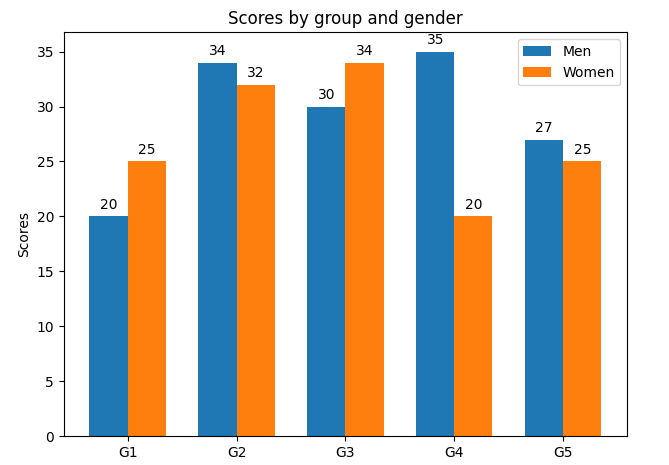
\includegraphics[height = \rowheight]{img/matplotlib-graph.png}
        \end{cell}
        \begin{cell}{0.079}
          ~
        \end{cell}
        \begin{cell}{0.473}
          \centering
          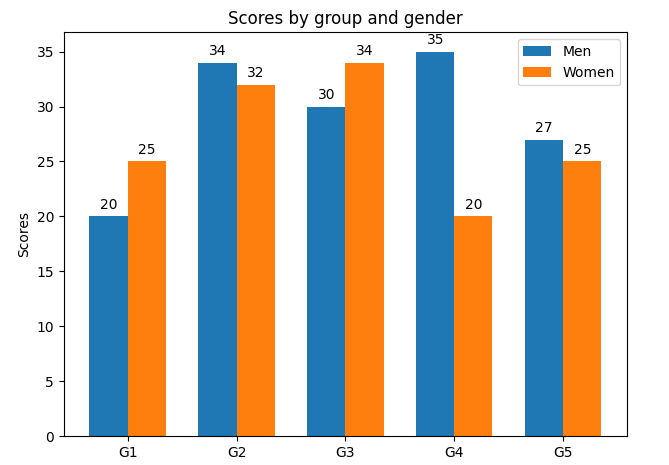
\includegraphics[height = \rowheight]{img/matplotlib-graph.png}
        \end{cell}
      \end{row}
    \end{gridlayout}
\end{frame}



\begin{frame}{Title of frame 4}
  \begin{imaths}
    a + \int \mathbf{b^4} + \frac{c}{d}
  \end{imaths}
\end{frame}



\begin{frame}{Title of frame 5}

\end{frame}

%%%%%%%%%%%%%%%%%%%%%%%%%%%%%%%% STOP EDITING HERE


\end{document}